\documentclass[
11pt, % The default document font size, options: 10pt, 11pt, 12pt
codirector, % Uncomment to add a codirector to the title page
]{charter} 




% El títulos de la memoria, se usa en la carátula y se puede usar el cualquier lugar del documento con el comando \ttitle
%\titulo{Título del proyecto} 
\titulo{Dispositivo para pruebas de comunicación con satélites} 

% Nombre del posgrado, se usa en la carátula y se puede usar el cualquier lugar del documento con el comando \degreename
\posgrado{Carrera de Especialización en Sistemas Embebidos} 
%\posgrado{Carrera de Especialización en Internet de las Cosas} 
%\posgrado{Carrera de Especialización en Intelegencia Artificial}
%\posgrado{Maestría en Sistemas Embebidos} 
%\posgrado{Maestría en Internet de las cosas}

% Tu nombre, se puede usar el cualquier lugar del documento con el comando \authorname
\autor{Facundo G. Colavitte} 

% El nombre del director y co-director, se puede usar el cualquier lugar del documento con el comando \supname y \cosupname y \pertesupname y \pertecosupname
\director{\textcolor{red}{Director a definir}}
\pertenenciaDirector{\textcolor{red}{pertenencia}} 
% FIXME:NO IMPLEMENTADO EL CODIRECTOR ni su pertenencia
%\codirector{John Doe} % para que aparezca en la portada se debe descomentar la opción codirector en el documentclass
%\pertenenciaCoDirector{FIUBA}

% Nombre del cliente, quien va a aprobar los resultados del proyecto, se puede usar con el comando \clientename y \empclientename
\cliente{David Vilaseca}
\empresaCliente{Satellogic}

% Nombre y pertenencia de los jurados, se pueden usar el cualquier lugar del documento con el comando \jurunoname, \jurdosname y \jurtresname y \perteunoname, \pertedosname y \pertetresname.
\juradoUno{Nombre y Apellido (1)}
\pertenenciaJurUno{pertenencia (1)} 
\juradoDos{Nombre y Apellido (2)}
\pertenenciaJurDos{pertenencia (2)}
\juradoTres{Nombre y Apellido (3)}
\pertenenciaJurTres{pertenencia (3)}
 
\fechaINICIO{20 de octubre de 2022}		%Fecha de inicio de la cursada de GdP \fechaInicioName
\fechaFINALPlan{8 de diciembre de 2022} 	%Fecha de final de cursada de GdP
\fechaFINALTrabajo{21 de agosto de 2023}	%Fecha de defensa pública del trabajo final


\begin{document}

\maketitle
\thispagestyle{empty}
\pagebreak


\thispagestyle{empty}
{\setlength{\parskip}{0pt}
\tableofcontents{}
}
\pagebreak


\section*{Registros de cambios}
\label{sec:registro}


\begin{table}[ht]
\label{tab:registro}
\centering
\begin{tabularx}{\linewidth}{@{}|c|X|c|@{}}
\hline
\rowcolor[HTML]{C0C0C0} 
Revisión & \multicolumn{1}{c|}{\cellcolor[HTML]{C0C0C0}Detalles de los cambios realizados} & Fecha      \\ \hline
v0.0      & Creación del documento                                 &\fechaInicioName \\ \hline
v1.0      & Se completa hasta el punto 5 inclusive                 & 03 de noviembre de 2022 \\ \hline
v2.0      & Se completa hasta el punto 9 inclusive                & 10 de noviembre de 2022 \\ \hline
%v3.0      & Se completa hasta el punto 12 inclusive               & 17 de noviembre de 2022 \\ \hline
%v4.0      & Se completa el plan	                               & 24 de noviembre de 2022 \\ \hline
\end{tabularx}
\end{table}

\pagebreak



\section*{Acta de constitución del proyecto}
\label{sec:acta}

\begin{flushright}
Buenos Aires, \fechaInicioName
\end{flushright}

\vspace{2cm}

Por medio de la presente se acuerda con el Ing. \authorname\hspace{1px} que su Trabajo Final de la \degreename\hspace{1px} se titulará ``\ttitle'', consistirá esencialmente en el diseño de un prototipo modular, versátil, para realizar pruebas de comunicación unidireccional con satélites de órbita baja usando un módulo LoRa, y tendrá un presupuesto preliminar estimado de 600 hs de trabajo y \$30.000, con fecha de inicio \fechaInicioName\hspace{1px} y fecha de presentación pública \fechaFinalName.

Se adjunta a esta acta la planificación inicial.

\vfill

% Esta parte se construye sola con la información que hayan cargado en el preámbulo del documento y no debe modificarla
\begin{table}[ht]
\centering
\begin{tabular}{ccc}
\begin{tabular}[c]{@{}c@{}}Ariel Lutenberg \\ Director posgrado FIUBA\end{tabular} & \hspace{2cm} & \begin{tabular}[c]{@{}c@{}}\clientename \\ \empclientename \end{tabular} \vspace{2.5cm} \\ 
\multicolumn{3}{c}{\begin{tabular}[c]{@{}c@{}} \supname \\ Director del Trabajo Final\end{tabular}} \vspace{2.5cm} \\
%\begin{tabular}[c]{@{}c@{}}\jurunoname \\ Jurado del Trabajo Final\end{tabular}     &  & \begin{tabular}[c]{@{}c@{}}\jurdosname\\ Jurado del Trabajo Final\end{tabular}  \vspace{2.5cm}  \\
%\multicolumn{3}{c}{\begin{tabular}[c]{@{}c@{}} \jurtresname\\ Jurado del Trabajo Final\end{tabular}} \vspace{.5cm}                                                                     
\end{tabular}
\end{table}




\section{1. Descripción técnica-conceptual del proyecto a realizar}
\label{sec:descripcion}

La realización del siguiente proyecto se basa en la construcción de un prototipo para realizar pruebas de comunicación unidireccional con satélites de la empresa Satellogic. Esta última posee actualmente satélites de órbita baja para mapeo de la superficie terrestre mediante sistema de capturas de imágenes. Su objetivo es agregar a su cartera de servicios satelitales la posibilidad de recibir información de dispositivos IoT en tierra para ofrecerle una alternativa a los medios de comunicación tradicionales. Por esta razón, se realizará un dispositivo modular, versátil, que permita enviar datos tomados en tierra a los satélite en órbita baja para realizar las pruebas pertinentes.

La idea no es probar con un satélite real ya que el uso de comunicación por LorRa es una propuesta de la empresa dado que ciertos módulos trabajan a frecuencias similares. Es por esto que el proyecto será validado por la comunicación entre dos prototipos en tierra que cumplan con las requerimientos teóricos que Satellogic solicita. En caso de realizarse una prueba con el satélite la no recepción del mensaje no involucrará fallas en el diseño del sistema.
Pese a esto, el dispositivo deberá ser diseñado considerando que su finalidad sea una comunicación desde la tierra hacia el satélite a través de un módulo LoRa de forma unidireccional a una frecuencia cercana a 920 MHz. Los datos a enviar por el prototipo deben poder ser tomados por USB y WiFi.


Como se observa en la figura \ref{fig:diagBloques}, el dispositivo posee:
\begin{itemize}
	\item Un puerto de conexión USB para comunicación con ordenadores locales.
	\item Conexión WiFi para ser manejado de forma remota.
	\item Alimentación externa.
	\item Puerto de conexión para antena tipo QFH.
\end{itemize}

\begin{figure}[htpb]
\centering 
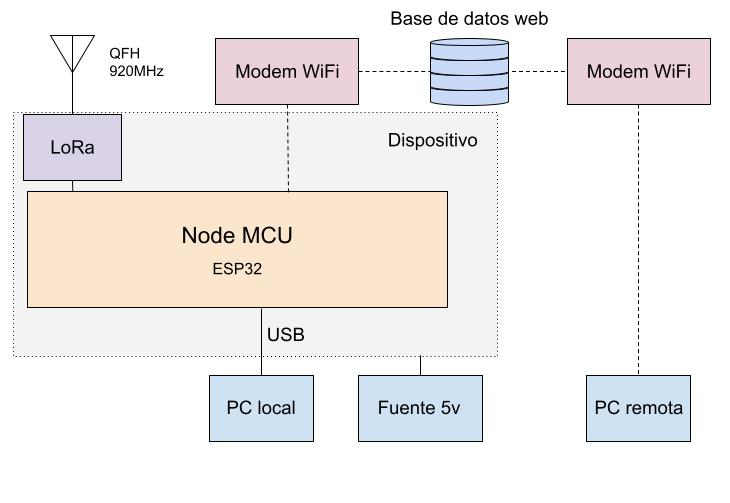
\includegraphics[width=.8\textwidth]{./Figuras/Diagrama de bloques.jpg}
\caption{Diagrama en bloques del sistema.}
\label{fig:diagBloques}
\end{figure}

\vspace{25px}

El presente proyecto se destaca en la incorporación de conexión WiFi para recepción de los datos. Dado que es condición necesaria que la comunicación se realice a cielo abierto, el contar con WiFi permite establecer esta comunicación aún cuando haya condiciones climáticas desfavorables para la presencia del usuario.

\textcolor{red}{
En el mercado no existe a día de hoy un dispositivo específico para tal finalidad por lo que no se presenta sistemas comerciales similares de los cuales diferenciarse.
}

\section{2. Identificación y análisis de los interesados}
\label{sec:interesados}


\begin{table}[ht]
%\caption{Identificación de los interesados}
%\label{tab:interesados}
\begin{tabularx}{\linewidth}{@{}|l|X|X|l|@{}}
\hline
\rowcolor[HTML]{C0C0C0} 
Rol           & Nombre y Apellido & Organización 	& Puesto 	\\ \hline
Auspiciante   & \clientename      &\empclientename	& Director de Research 	\\ \hline
Cliente       & \clientename      &\empclientename	& Director de Research 	\\ \hline
Responsable   & \authorname       & FIUBA        	& Alumno 	\\ \hline
Colaboradores & Scasserra Marco   & FIUBA         	& Alumno   	\\ \hline
Orientador    & \supname	      & \pertesupname 	& Director Trabajo final \\ \hline
Usuario final & Pega Luciano      &\empclientename	& Ingeniero en Research  \\ \hline
\end{tabularx}
\end{table}


\begin{itemize}
	\item Pega Luciano: trabaja en la misma área que el cliente. Puede responder preguntas de requerimientos técnicos y validar el proyecto.
	\item Scasserra Marco: trabaja en un proyecto final del CESE de la misma temática para el mismo cliente.
	\item \supname: posee experiencia en módulos LoRa y sistemas de almacenamiento de energía.
\end{itemize}



\section{3. Propósito del proyecto}
\label{sec:proposito}

El propósito del proyecto es diseñar un dispositivo que permita realizar pruebas de comunicación con satélites de órbita baja para una posterior implementación de dicha tecnología en dispositivos IoT. El prototípo debe ser versátil y estar conformado principalmente por módulos electrónicos comerciales para facilitar su posterior modificación según lo ameriten las pruebas.


\section{4. Alcance del proyecto}
\label{sec:alcance}

El proyecto incluye:
\begin{itemize}
	\item Un prototipo físico con el firmware cargado.
	\item Código fuente del firmware.
	\item Esquemático del hardware.
	\item Sistema de alimentación.
\end{itemize}
El proyecto no incluye:
\begin{itemize}
	\item Dispositivo comercial.
	\item Script que decodifica la señal IQ recibida en el satélite.
	\item Software de escritorio para envío de datos al dispositivo.
	\item Montaje del dispositivo.
\end{itemize}


\section{5. Supuestos del proyecto}
\label{sec:supuestos}

Para el desarrollo del presente proyecto se supone que:

\begin{itemize}
	\item Si dos dispositivos se pueden comunicar en tierra por medio de módulos LoRa la señal puede ser recibida por un satélite que esté dentro del alcance del conjunto módulo LoRa-Antena.
	\item Disponibilidad de todos los materiales necesaros para la construcción del prototípo por parte de la empresa Satellogic. Los mismos se detallarán en la Lista de materiales conforme se realice el proyecto.
	\item No se presentaran retenciones a importaciones de los materiales necesarios que dificulten su disponibilidad.
	\item Se dispondrá de al menos 80 horas mensuales en promedio para dedicar al proyecto.
	\item Los materiales necesarios para las pruebas y construcción de prototipos se dispondran en un tiempo no mayor a dos semanas tras solicitarlos.
\end{itemize}

\section{6. Requerimientos}
\label{sec:requerimientos}

\begin{enumerate}
	\item Requerimientos funcionales
		\begin{enumerate}
			\item El dispositivo debe ser simple de replicar, preferentemente ensamblable con módulos comerciales.
			\item El dispositivo debe ser versátil, pudiéndose adaptar a distintas \textcolor{red}{características de comunicación} de forma simple.
			\item El módulo LoRa debe ser un E22 900M30S de EBYTE (30 dBm).
			\item El dispositivo debe poder ser lo más cercano posible a la metodología "plug 'n play".
			\item El usuario debe poder enviar mensajes por medio de un terminal serie.
		\end{enumerate}
	\item Requerimientos de documentación
		\begin{enumerate}
			\item Manual de usuario.
			\item Documentación del firmware.
		\end{enumerate}
	\item Requerimiento de testing
		\begin{enumerate}
			\item Se debe poder establecer comunicación por LoRa con otro dispositivo en tierra que posea igual módulo con una distancia menor a un metro.
		\end{enumerate}
	\textcolor{red}{
	\item Requerimientos de la interfaz...
	\item Requerimientos interoperabilidad...
	}
\end{enumerate}

\section{7. Historias de usuarios (\textit{Product backlog})}
\label{sec:backlog}

\begin{itemize}
	\item “Como usuario, quiero que el dispositivo sea compacto, robusto y ligero, de modo de poder llevarlo al lugar donde debe realizarse el experimento.”
	\item “Como usuario, quiero que el dispositivo se conecte a WiFi para poder operarlo de manera remota.“
	\item “Como usuario, quiero que la interfaz de comunicación sea CLI, para que la operación sea ágil.”
	\item “Como usuario, quiero que el dispositivo cuente con un conector de RF, de modo de poder elegir distintos tipos de antenas, o incluso agregar una etapa de amplificación adicional, de ser necesario.”
	\item “Como usuario, quiero que el dispositivo sea suficientemente pequeño como para poder integrarse en un gabinete estanco, lo cual permitiría a operación en intemperie.”
\end{itemize}


\begin{consigna}{red}
Descripción: En esta sección se deben incluir las historias de usuarios y su ponderación (\textit{history points}). Recordar que las historias de usuarios son descripciones cortas y simples de una característica contada desde la perspectiva de la persona que desea la nueva capacidad, generalmente un usuario o cliente del sistema. La ponderación es un número entero que representa el tamaño de la historia comparada con otras historias de similar tipo.

El formato propuesto es: "como [rol] quiero [tal cosa] para [tal otra cosa]."

Se debe indicar explícitamente el criterio para calcular los \textit{story points} de cada historia
\end{consigna}

\section{8. Entregables principales del proyecto}
\label{sec:entregables}

Los entregables del proyecto son:
\begin{itemize}
	\item Manual de usuario.
	\item Diagrama de circuitos esquemáticos.
	\item Código fuente del firmware.
	\item Archivo Gerber.
	\item Lista de componentes electrónicos.
	\item Un prototipo funcional.
\end{itemize}



\section{9. Desglose del trabajo en tareas}
\label{sec:wbs}

\begin{enumerate}
\item Recopilación general de información sobre el proyecto (50 hs)
	\begin{enumerate}
	\item Investigar sobre tecnología WiFi. (10 hs)
	\item Investigar sobre tecnología LoRa. (10 hs)
	\item Investigar específica sobre módulo LoRa E22. (10 hs)
	\item Investigar Investigación sobre antenas QFH. (10 hs)
	\item Investigar Investigación sobre base de datos web. (10 hs)
	\end{enumerate}
\item Planificación del proyecto (30 hs)
	\begin{enumerate}
	\item Realizar planificación del proyecto (30 hs)
	\item Tarea 2 (tantas hs)
	\item Tarea 3 (tantas hs)
	\end{enumerate}
\item Hardware (140 hs)
	\begin{enumerate}
	\item Selección de componentes (12 hs)
	\item Diseño del circuito esquemático (28 hs)
	\item Diseño del PCB (30 hs)
	\item Fabricación y ensamblado del PCB (30 hs)
	\item Pruebas y validación del hardware (40 hs)
	\end{enumerate}
\item Firmware (\textcolor{red}{---} hs)
	\begin{enumerate}
	\item Desarrollo de arquitectura del firmware (16 hs)
	\item Diseño de firmware (32 hs)
	\item Desarrollo de pruebas para firmware (32 hs)
	\item Programación del firmware (40 hs)
	\item Verificación y validación del firmware (24 hs)
	\end{enumerate}
\item \textcolor{red}{???? (--- hs)}
	\begin{enumerate}
	\item Desarrollo de arquitectura del firmware (16 hs)
	\item Diseño de firmware (32 hs)
	\item Desarrollo de pruebas para firmware (32 hs)
	\item Programación del firmware (40 hs)
	\item Verificación y validación del firmware (24 hs)
	\end{enumerate}
\item Diseño del gabinete (40 hs)
	\begin{enumerate}
	\item Diseño de la carcasa de los sensores (20 hs)
	\item Armado del gabinete de los nodos sensores (20 hs)
	\end{enumerate}
\item Procesos finales (\textcolor{red}{---} hs)
	\begin{enumerate}
	\item Elaboración del informe de avance (20 hs)
	\item Evaluación de requerimientos (25 hs)
	\item Elaboración de la memoria del proyecto (40 hs)
	\item Preparación de la presentación final (35 hs)
	\end{enumerate}
\end{enumerate}



Cantidad total de horas: (tantas hs)

\begin{consigna}{red}
El WBS debe tener relación directa o indirecta con los requerimientos.  Son todas las actividades que se harán en el proyecto para dar cumplimiento a los requerimientos. Se recomienda mostrar el WBS mediante una lista indexada:

\begin{enumerate}
\item Grupo de tareas 1
	\begin{enumerate}
	\item Tarea 1 (tantas hs)
	\item Tarea 2 (tantas hs)
	\item Tarea 3 (tantas hs)
	\end{enumerate}
\item Grupo de tareas 2
	\begin{enumerate}
	\item Tarea 1 (tantas hs)
	\item Tarea 2 (tantas hs)
	\item Tarea 3 (tantas hs)
	\end{enumerate}
\item Grupo de tareas 3
	\begin{enumerate}
	\item Tarea 1 (tantas hs)
	\item Tarea 2 (tantas hs)
	\item Tarea 3 (tantas hs)
	\item Tarea 4 (tantas hs)
	\item Tarea 5 (tantas hs)
	\end{enumerate}
\end{enumerate}

Cantidad total de horas: (tantas hs)

Se recomienda que no haya ninguna tarea que lleve más de 40 hs. 

\end{consigna}

\section{10. Diagrama de Activity On Node}
\label{sec:AoN}

\begin{consigna}{red}
Armar el AoN a partir del WBS definido en la etapa anterior. 

%La figura \ref{fig:AoN} fue elaborada con el paquete latex tikz y pueden consultar la siguiente referencia \textit{online}:

%\url{https://www.overleaf.com/learn/latex/LaTeX_Graphics_using_TikZ:_A_Tutorial_for_Beginners_(Part_3)\%E2\%80\%94Creating_Flowcharts}

\end{consigna}

\begin{figure}[htpb]
\centering 
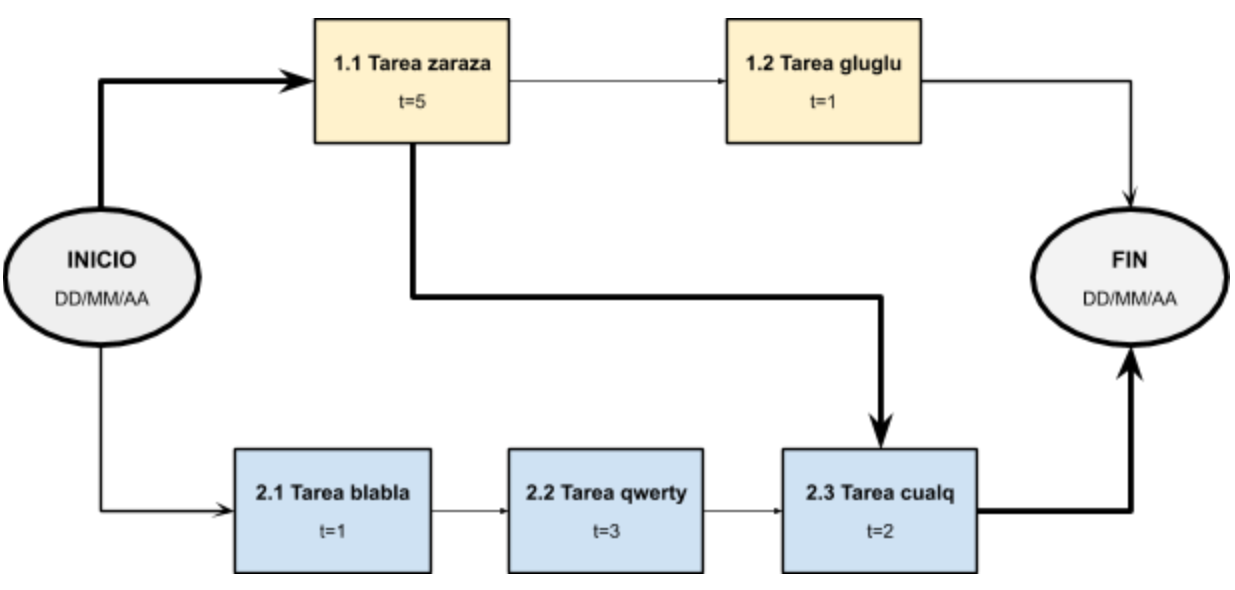
\includegraphics[width=.8\textwidth]{./Figuras/AoN.png}
\caption{Diagrama en \textit{Activity on Node}}
\label{fig:AoN}
\end{figure}

Indicar claramente en qué unidades están expresados los tiempos.
De ser necesario indicar los caminos semicríticos y analizar sus tiempos mediante un cuadro.
Es recomendable usar colores y un cuadro indicativo describiendo qué representa cada color, como se muestra en el siguiente ejemplo:



\section{11. Diagrama de Gantt}
\label{sec:gantt}

\begin{consigna}{red}

Existen muchos programas y recursos \textit{online} para hacer diagramas de gantt, entre los cuales destacamos:

\begin{itemize}
\item Planner
\item GanttProject
\item Trello + \textit{plugins}. En el siguiente link hay un tutorial oficial: \\ \url{https://blog.trello.com/es/diagrama-de-gantt-de-un-proyecto}
\item Creately, herramienta online colaborativa. \\\url{https://creately.com/diagram/example/ieb3p3ml/LaTeX}
\item Se puede hacer en latex con el paquete \textit{pgfgantt}\\ \url{http://ctan.dcc.uchile.cl/graphics/pgf/contrib/pgfgantt/pgfgantt.pdf}
\end{itemize}

Pegar acá una captura de pantalla del diagrama de Gantt, cuidando que la letra sea suficientemente grande como para ser legible. 
Si el diagrama queda demasiado ancho, se puede pegar primero la ``tabla'' del Gantt y luego pegar la parte del diagrama de barras del diagrama de Gantt.

Configurar el software para que en la parte de la tabla muestre los códigos del EDT (WBS).\\
Configurar el software para que al lado de cada barra muestre el nombre de cada tarea.\\
Revisar que la fecha de finalización coincida con lo indicado en el Acta Constitutiva.

En la figura \ref{fig:gantt}, se muestra un ejemplo de diagrama de gantt realizado con el paquete de \textit{pgfgantt}. En la plantilla pueden ver el código que lo genera y usarlo de base para construir el propio.

\begin{figure}[htbp]
\begin{center}
\begin{ganttchart}{1}{12}
  \gantttitle{2020}{12} \\
  \gantttitlelist{1,...,12}{1} \\
  \ganttgroup{Group 1}{1}{7} \\
  \ganttbar{Task 1}{1}{2} \\
  \ganttlinkedbar{Task 2}{3}{7} \ganttnewline
  \ganttmilestone{Milestone o hito}{7} \ganttnewline
  \ganttbar{Final Task}{8}{12}
  \ganttlink{elem2}{elem3}
  \ganttlink{elem3}{elem4}
\end{ganttchart}
\end{center}
\caption{Diagrama de gantt de ejemplo}
\label{fig:gantt}
\end{figure}


\begin{landscape}
\begin{figure}[htpb]
\centering 
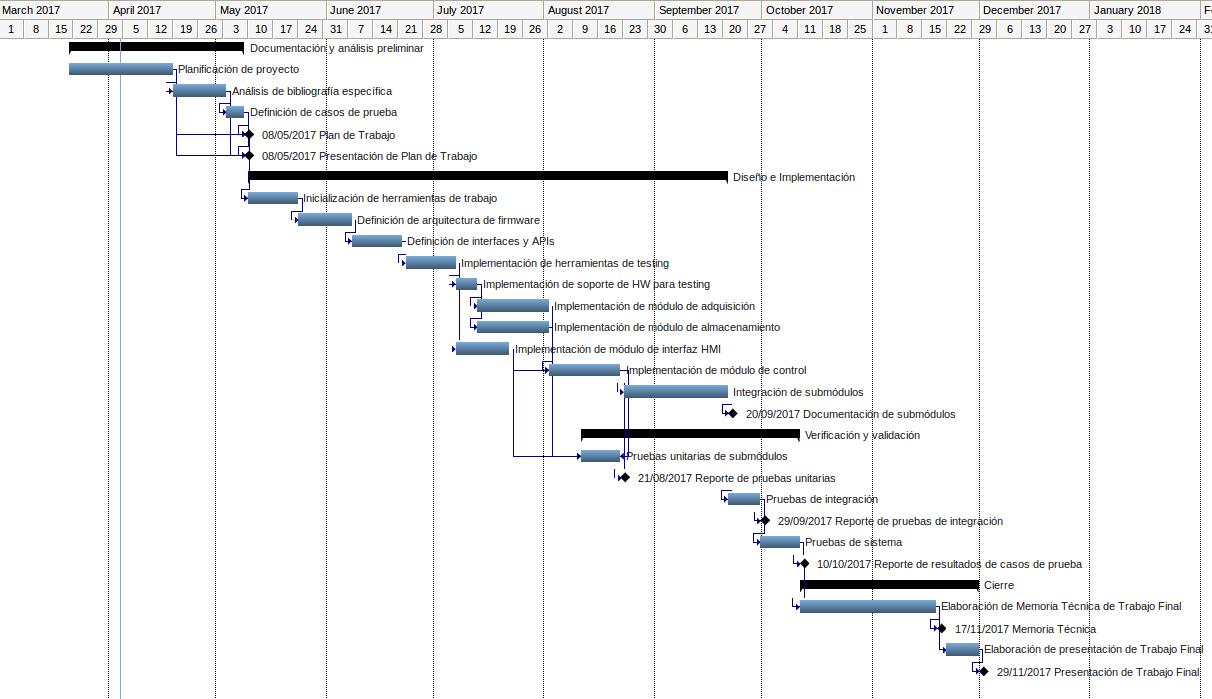
\includegraphics[height=.85\textheight]{./Figuras/Gantt-2.png}
\caption{Ejemplo de diagrama de Gantt rotado}
\label{fig:diagGantt}
\end{figure}

\end{landscape}

\end{consigna}


\section{12. Presupuesto detallado del proyecto}
\label{sec:presupuesto}

\begin{consigna}{red}
Si el proyecto es complejo entonces separarlo en partes:
\begin{itemize}
	\item Un total global, indicando el subtotal acumulado por cada una de las áreas.
	\item El desglose detallado del subtotal de cada una de las áreas.
\end{itemize}

IMPORTANTE: No olvidarse de considerar los COSTOS INDIRECTOS.

\end{consigna}

\begin{table}[htpb]
\centering
\begin{tabularx}{\linewidth}{@{}|X|c|r|r|@{}}
\hline
\rowcolor[HTML]{C0C0C0} 
\multicolumn{4}{|c|}{\cellcolor[HTML]{C0C0C0}COSTOS DIRECTOS} \\ \hline
\rowcolor[HTML]{C0C0C0} 
Descripción &
  \multicolumn{1}{c|}{\cellcolor[HTML]{C0C0C0}Cantidad} &
  \multicolumn{1}{c|}{\cellcolor[HTML]{C0C0C0}Valor unitario} &
  \multicolumn{1}{c|}{\cellcolor[HTML]{C0C0C0}Valor total} \\ \hline
 &
  \multicolumn{1}{c|}{} &
  \multicolumn{1}{c|}{} &
  \multicolumn{1}{c|}{} \\ \hline
 &
  \multicolumn{1}{c|}{} &
  \multicolumn{1}{c|}{} &
  \multicolumn{1}{c|}{} \\ \hline
\multicolumn{1}{|l|}{} &
   &
   &
   \\ \hline
\multicolumn{1}{|l|}{} &
   &
   &
   \\ \hline
\multicolumn{3}{|c|}{SUBTOTAL} &
  \multicolumn{1}{c|}{} \\ \hline
\rowcolor[HTML]{C0C0C0} 
\multicolumn{4}{|c|}{\cellcolor[HTML]{C0C0C0}COSTOS INDIRECTOS} \\ \hline
\rowcolor[HTML]{C0C0C0} 
Descripción &
  \multicolumn{1}{c|}{\cellcolor[HTML]{C0C0C0}Cantidad} &
  \multicolumn{1}{c|}{\cellcolor[HTML]{C0C0C0}Valor unitario} &
  \multicolumn{1}{c|}{\cellcolor[HTML]{C0C0C0}Valor total} \\ \hline
\multicolumn{1}{|l|}{} &
   &
   &
   \\ \hline
\multicolumn{1}{|l|}{} &
   &
   &
   \\ \hline
\multicolumn{1}{|l|}{} &
   &
   &
   \\ \hline
\multicolumn{3}{|c|}{SUBTOTAL} &
  \multicolumn{1}{c|}{} \\ \hline
\rowcolor[HTML]{C0C0C0}
\multicolumn{3}{|c|}{TOTAL} &
   \\ \hline
\end{tabularx}%
\end{table}


\section{13. Gestión de riesgos}
\label{sec:riesgos}

\begin{consigna}{red}
a) Identificación de los riesgos (al menos cinco) y estimación de sus consecuencias:
 
Riesgo 1: detallar el riesgo (riesgo es algo que si ocurre altera los planes previstos de forma negativa)
\begin{itemize}
	\item Severidad (S): mientras más severo, más alto es el número (usar números del 1 al 10).\\
	Justificar el motivo por el cual se asigna determinado número de severidad (S).
	\item Probabilidad de ocurrencia (O): mientras más probable, más alto es el número (usar del 1 al 10).\\
	Justificar el motivo por el cual se asigna determinado número de (O). 
\end{itemize}   

Riesgo 2:
\begin{itemize}
	\item Severidad (S): 
	\item Ocurrencia (O):
\end{itemize}

Riesgo 3:
\begin{itemize}
	\item Severidad (S): 
	\item Ocurrencia (O):
\end{itemize}


b) Tabla de gestión de riesgos:      (El RPN se calcula como RPN=SxO)

\begin{table}[htpb]
\centering
\begin{tabularx}{\linewidth}{@{}|X|c|c|c|c|c|c|@{}}
\hline
\rowcolor[HTML]{C0C0C0} 
Riesgo & S & O & RPN & S* & O* & RPN* \\ \hline
       &   &   &     &    &    &      \\ \hline
       &   &   &     &    &    &      \\ \hline
       &   &   &     &    &    &      \\ \hline
       &   &   &     &    &    &      \\ \hline
       &   &   &     &    &    &      \\ \hline
\end{tabularx}%
\end{table}

Criterio adoptado: 
Se tomarán medidas de mitigación en los riesgos cuyos números de RPN sean mayores a...

Nota: los valores marcados con (*) en la tabla corresponden luego de haber aplicado la mitigación.

c) Plan de mitigación de los riesgos que originalmente excedían el RPN máximo establecido:
 
Riesgo 1: plan de mitigación (si por el RPN fuera necesario elaborar un plan de mitigación).
  Nueva asignación de S y O, con su respectiva justificación:
  - Severidad (S): mientras más severo, más alto es el número (usar números del 1 al 10).
          Justificar el motivo por el cual se asigna determinado número de severidad (S).
  - Probabilidad de ocurrencia (O): mientras más probable, más alto es el número (usar del 1 al 10).
          Justificar el motivo por el cual se asigna determinado número de (O).

Riesgo 2: plan de mitigación (si por el RPN fuera necesario elaborar un plan de mitigación).
 
Riesgo 3: plan de mitigación (si por el RPN fuera necesario elaborar un plan de mitigación).

\end{consigna}


\section{14. Gestión de la calidad}
\label{sec:calidad}

\begin{consigna}{red}
Para cada uno de los requerimientos del proyecto indique:
\begin{itemize} 
\item Req \#1: copiar acá el requerimiento.

\begin{itemize}
	\item Verificación para confirmar si se cumplió con lo requerido antes de mostrar el sistema al cliente. Detallar 
	\item Validación con el cliente para confirmar que está de acuerdo en que se cumplió con lo requerido. Detallar  
\end{itemize}

\end{itemize}

Tener en cuenta que en este contexto se pueden mencionar simulaciones, cálculos, revisión de hojas de datos, consulta con expertos, mediciones, etc.  Las acciones de verificación suelen considerar al entregable como ``caja blanca'', es decir se conoce en profundidad su funcionamiento interno.  En cambio, las acciones de validación suelen considerar al entregable como ``caja negra'', es decir, que no se conocen los detalles de su funcionamiento interno.

\end{consigna}

\section{15. Procesos de cierre}    
\label{sec:cierre}

\begin{consigna}{red}
Establecer las pautas de trabajo para realizar una reunión final de evaluación del proyecto, tal que contemple las siguientes actividades:

\begin{itemize}
	\item Pautas de trabajo que se seguirán para analizar si se respetó el Plan de Proyecto original:
	 - Indicar quién se ocupará de hacer esto y cuál será el procedimiento a aplicar. 
	\item Identificación de las técnicas y procedimientos útiles e inútiles que se emplearon, y los problemas que surgieron y cómo se solucionaron:
	 - Indicar quién se ocupará de hacer esto y cuál será el procedimiento para dejar registro.
	\item Indicar quién organizará el acto de agradecimiento a todos los interesados, y en especial al equipo de trabajo y colaboradores:
	  - Indicar esto y quién financiará los gastos correspondientes.
\end{itemize}

\end{consigna}


\end{document}
